%Phase3
\chapter{Code Generation}
Code generation is the phase in which the object code is generated, the process and considerations this entails are covered in this chapter.
Object code is the output of the compiler.
Once the source code has passed through syntax analysis and contextual analysis without errors it has been validated and the compiler can proceed with generating the object code.
In the case of this compiler the object code is OpenCL C, as a result one or more compilers beyond this one are required to eventually end up with machine code that can be executed.\todo{more compilers? - e.g. vi bruger vores egen og gcc - Marc}
The object code is OpenCL C this means that tasks such as instruction selection and scheduling as well as register allocation will be handled by the compiler which will compile the OpenCL C code rather than \gls{gamble}.\todo{Håndterer compileren scheduling ????? - Søren - Instruction scheduling var en af de nævnte ting fra SPO kurset som man på lavniveau håndtere ja - Marc .. instruction scheduling er jo hvilken rækkefølge en given sekvens af instruktioner udføres i, ikke hvilken process har adgang til CPUen på et givent tidspunkt. -- Troels}
Furthermore in the code generation phase optimisation of the object code also takes place, for \gls{gamble} this means to create object code which is quickly executed and utilises the \acrshort{gpu} for calculation that benefit from its use.\todo{er det ok at bruge optimisation her, vi code gen'er jo bare, det er jo ikke rigtig en optimering. ? :) - Søren - Men området er referet til som optimisation, det er også derfor der efter står hvad betydningen af optimisation er for gamble - Marc }
A state diagram showing the sub-phases of the code generation can be seen in \myref{fig:flowCodegen}.

\vspace{10pt}
\begin{figure}[h]
    \centering
    \begin{tikzpicture}[node distance = 3cm, auto]
        %\node (invi1) [invi, draw=none] {};
        %\node (ast) [lille, below=-0.35cm of invi1] {Abstract Syntax Tree};
        %\node (symboltable) [lille, minimum width=6.75cm, minimum height=2.4cm, right=2cm of invi1, fill=blue!10, label={[xshift=0cm, yshift=-1cm]Symbol Table}] {};
        %\node (scope) [lille, right=1.1cm of ast] {Scopechecker};
        %\node (type) [lille, right=0.7cm of scope] {Typechecker};
        %\node (dast) [lille, right=1.1cm of type] {Decorated Abstact Syntax Tree};

        %\node (error) [cloud, below=1cm of symboltable] {Error report};

        %\draw [arrow] (ast) -- (scope);
        %\draw [arrow] (scope) -- (type);
        %\draw [arrow] (type) -- (dast);
        %\draw [arrow,dashed] (scope) -- (error);
        %\draw [arrow,dashed] (type) -- (error);
        %\draw [arrow,dashed] (symboltable) -- (error);

        \node (dast) [lille, align=left] {Contextual \\Analysis Phase};
        \node (cgv) [lille, right=0.7cm of dast, align=left] {Code Generation \\Visitor};
        \node (copy) [lille, right=0.7cm of cgv] {Output \gls{opencl} C code};
        \node (error) [invi, draw=none, minimum width=2cm, right=1cm of copy, label={[xshift=40pt, yshift=-17pt]Finished Compilation}] {};

        \draw[black,fill=black, above=1cm of parser] (10.9,0) circle (1ex);
        \draw[black, above=1cm of parser] (10.9,0) circle (1.3ex); 

        \draw [arrow] (dast) -- (cgv);
        \draw [arrow] (cgv) -- (copy);
        \draw [arrow] (copy) -- (error);
    \end{tikzpicture}
    \caption{State diagram showing the modules of the code generation. } 
    \label{fig:flowCodegen}
\end{figure}
\vspace{-20pt}

\section{Design}
This section will cover the design of the code generator in the compiler, both the overall structure of the code generator and its requirements, but also its use of the \acrshort{gpu}.
Lastly it will present how the runtime of the programs could be made more efficient.
\subsubsection*{The Code Generator Visitor}
When the code generator is called, the \acrshort{ast} is used to accept a \texttt{CodeGeneratorVisitor} as seen on \myref{fig:CodeGeneratorVisitor}.

\begin{figure}[!ht]
\centering
 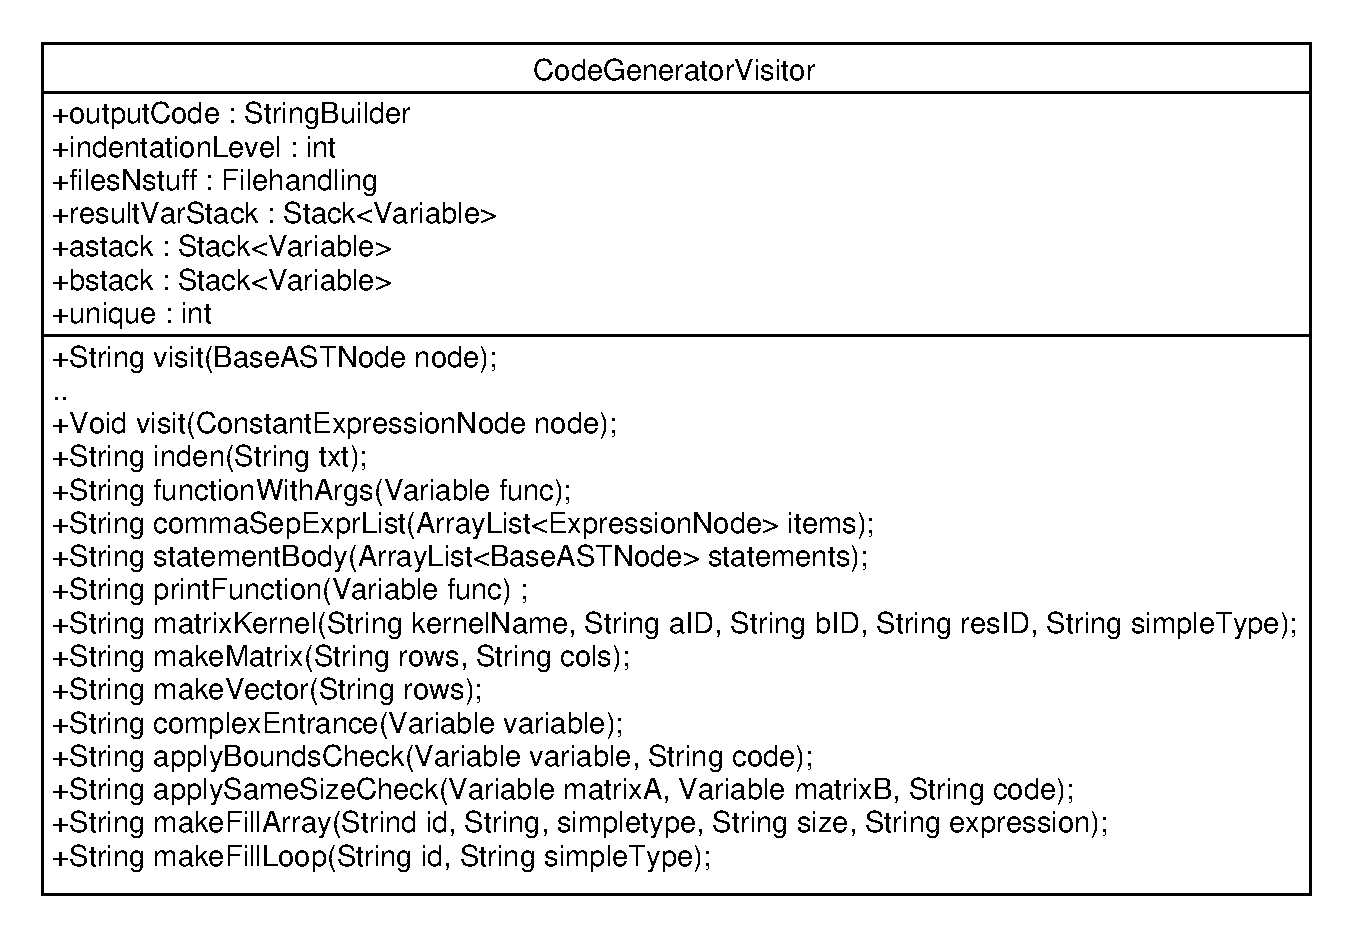
\includegraphics[width=0.8\textwidth]{figures/ClassDiagrams/CodeGeneratorCall.pdf}%trim=4cm 0cm 0cm 0cm, clip
\caption{A class diagram of \texttt{CodeGeneratorVisitor} showing the call from the code generator to the visitor which makes the string from the decorated \acrshort{ast}.}\label{fig:CodeGeneratorVisitor}
\vspace{-15pt}
\end{figure}

The visitor builds a string by traversing the nodes of the tree which will in the end be put into a file by the \texttt{CodeGenerator} class.
Some visit methods like a visit method for a \texttt{ConstantExpressionNode} returns a string while other methods instead directly appends to the string the visitor will return to the class \texttt{CodeGenerator}.
This string is then used as an argument in other visit methods e.g. \texttt{AssignmentNode} which then produces a string which is a statement that can be executed in C.
This string from \texttt{AssignmentNode} is  one of the string to be appended to the string containing the fully compiled program.
%%%%%%%%%%%%%%%%%%%%%%%%%%%%%%%%%%%%%%%%%%%%%%%%%%%%%%%%%%%%%%%%%%%%%%%%%%%%%%%%%%%%%%%%%%%%%%%%%%

As a result the information bubbles upwards from the leafs of the tree to the statementnodes.
The information is put in the correct statementnodes because the visitor pattern makes it possible to specify the route of traversal.
The \texttt{CodeGeneratorVisitor} also contains other methods for producing certain C constructions using the similar \gls{gamble} constructions found in the \acrshort{ast}.
These methods can also be seen on \myref{fig:CodeGeneratorVisitor}.
Some of these methods also make runtime checks of matrices, as matrices needs to be of compatible sizes for some of the operations which can be performed on a matrix, furthermore an index check is implemented such that an out of bounds error will occur if one tries to access memory beyond the bounds of the matrix.
When multiplying two matrices the left matrix of the multiplication has to be a $ N \times M $ while the right one has to be a $ M \times P $ matrix.
So the right matrix must have the same number of columns as the right matrix has rows.
If performing a matrix index multiplication, where every index is multiplied with the corresponding index of the the other matrix, the matrices have to have the same number of rows and columns.

These checks will be inserted as a surrounding if statement around the matrix calculations, so they have to pass these checks before the calculation will be done, if it does not pass an error will be printed.\todo{Der kommer da en fejl right ? - Søren}
The reason this is done at run-time instead of at compile-time is because the sizes of matrices can be dynamic, which results in making it impossible to check for this at compile-time.

When the string is complete it is written to a file called code.c, along with all the other files needed for running the code, e.g. the kernels used for performing computations on the \acrshort{gpu}.
The code.c file is structured so that it is a valid C program.
First off are the libraries included that C uses, then follows a list of prototypes which are all the \gls{gamble} functions translated into C code, both the user made and the ones from libraries.
After the prototypes the main function is made where the body consists of all the statements in the \gls{gamble} sourcecode translated into C.
After the main method all the implementations of the function prototypes are made.
\subsection*{GPU Usage}\label{GPUCode}
Since \gls{gamble} distances its programmers from directly controlling which computations are performed on the \acrshort{gpu}, determing what code to perform on the \acrshort{gpu} becomes a problem for the compiler to solve.\todo{task, lyder bedre eller hvad? MP. - tasks synes jeg ikke rigtigt passer en når det er hvilke kodesegmenter, måske operations hvis det skal ændres? - Marc}
To make this decision the compiler must know what kind of code performs faster on a \acrshort{gpu} than a \acrshort{cpu}.

From \myref{sec:comparch} it is clear that for it to make sense to move any computation to the \acrshort{gpu} it must be of significant size to make up for the overhead of moving data, and be executable in parallel.
If a computation is reliant on the outcome of other computations, the Fibonacci function as an example, moving it to the \acrshort{gpu} would be a significant decrease in performance compared to a \acrshort{cpu}.

Any code written in a recursive format will not be run on the \acrshort{gpu}. 
Furthermore due to the overhead in data transfer, only computations requiring a significant amount of operations to be performed should be executed on the \acrshort{gpu} as \myref{image:benchmark} shows.
Therefore statements which only contain simple data types, i.e. integers, floats and booleans, are performed on the \acrshort{cpu}.
An example could be \texttt{value = value1 + value2}, where all types are integers.
%Therefore statements not containing complex data types, i.e. statements with no vector or matrix arithmetics, are also performed on the \acrshort{gpu}.

However statements that do include matrix or vector arithmetics will be performed on the \acrshort{gpu}.
An example could be matrix multiplication.
Now it is entirely possible to make a matrix multiplication of a $2\times2$ matrix, which would be so small that the overhead of data transfer is more expensive than simply computing on the \acrshort{cpu}. \todo{Det er jo ikke kune data overførslen som koster tid? Der er også JIT af kernel i nogle cases (se alle). -- Troels}
However to simplify the code generation it has been chosen that all matrix or vector calculations, are to be done on the \acrshort{gpu}.
This is not always the best choice, as \myref{sec:comparch} clearly shows, but it requires less analysis of the code given, furthermore as mentioned in \myref{sec:phil} \gls{gamble} uses the \acrshort{gpu} to gain computational power for performing already developed algorithms on data sets big enough to see an improvement in execution time.
Also even if smaller matrices are being computed, the increase in runtime is significantly less than the decrease for just a single bigger matrix operation, as can be seen on \myref{fig:test_results}.
\todo[inline]{Måske nævne vi hellere vil flytte små matricer på gpu, end at beholde store på cpuen? MP - God ide, den tid det tager at flytte en lille matrix til GPU er heller ikke så stor som det man spare på at flytte store matricer til gpu'en. - Søren - Som ovenstående? - Marc}


\subsection*{Runtime Efficiency}\label{subsec:runtime}
A consideration in a compiler is the performance or efficiency of its output. 
Rather than blindly translating the source code, translating to something more efficient is a subproblem in compiler optimisation.\todo{Farlig sætning iflg. Thomas:p - Søren - Men dette er fagtermet, sætningen lige efter specificere dette og nævner også hvorfor det ikke referes til som optimisation fremadrettet, synes den er meget let at komme ud af - Marc}
Optimisation is however a nonspecific and absolute word, therefore in \gls{gamble} we will instead be referring to the problem as improving or increasing runtime efficiency.
Runtime efficiency entails considerations of memory allocation, pipelining, parallelization etc. which may have an impact on execution time.
To do an efficient and complete analysis of how to increase runtime efficiency, information of the situation in a given program is required.
This is where \gls{gamble} is at a disadvantage. 
\gls{gamble} distances its programmers from controlling where the code is performed and instead does so seamlessly.
Information about how e.g. a for-loop could be transformed into a kernel does not exist in \gls{gamble} which makes it difficult to do this.\todo{er ikke helt med her? MP - Vi ved ikke om et for-loop er paralleliser bart eller ej ud fra informationen i AST'et - Marc ... Her kunne en pfor-løkke være brugbar. -- Troels}
The seamless use of the \acrshort{gpu} means that certain information is nonexistent and therefore all computations may not be candidates for improving its runtime efficiency, this is one of the trade-offs \gls{gamble} makes, meaning that simplicity of the language is valued over performance.\todo{Det her står imod principperne og er en farlig og dum sætning tbh. - Søren - Imod hvilke principper? - Marc}
If \gls{gamble} were to require more information, e.g. whether or not something is paralleliseable or ask the programmer to determine what type of \acrshort{gpu} memory should be used for each variable, the simplicity and seamless use of the \acrshort{gpu} would be lost.\todo{Tilføj evt:" and another language like Theano or directly programming OpenCL C might be a better choice." - Søren nb. theano er ikke et sprog -- Troels}

As previously mentioned due to the object code being OpenCL C certain considerations pertaining to instruction handling and register allocation etc. are not of interest for this compiler.
This is handled by using another compiler to compile the OpenCL C code into machine code, see \myref{ssub:makefile}. 
Instead to increase runtime efficiency the considerations concern when the \acrshort{gpu} should be used.\todo{What does this mean? - søren - At fremfor at håndtere performance i forhold til machine code skal det håndteres i forhold til OpenCL C - Marc}

As \gls{gamble} is attempting to seamlessly use the \acrshort{gpu} to increase performance, knowing when the use of the \acrshort{gpu} will actually be beneficial is an important point in the code generation process. \todo{Kom pludselig til at tænke på det jo ikke er vores sprog der bruger gpu'en men blot vores compiler der gør at vi gør det? Er det så forkert at skrive som her ? - Søren - Men det er som følge af vores sprog at det er seamless? kan ikke helt se hvad du vil skrive som alternativt, eller hvorfor det skulle være forkert - Marc}
As mentioned to do this efficiently, the compiler would require more information about the computations in a \gls{gamble} program than can be read from the syntax of \gls{gamble}.
Therefore it is decided that it is better to be sure that a computation can benefit from the \acrshort{gpu}, rather than risking moving computations that wont benefit with those that will.
As such only the operations that the project group knows have a possibility of benefiting from the parallel computational power of the \acrshort{gpu} will be executed on the \acrshort{gpu}.

%Knowing when to use GPU
Even though a computation can be parallelised, it does not necessarily mean it should be moved to the \acrshort{gpu}, as is evident in \myref{image:benchmark}.
This is an opportune moment for improving the runtime efficiency of the object code by using the \acrshort{gpu} only when it will be superior to the \acrshort{cpu} in regards to performance.
A possibility of doing so would be to analyse whether or not an instruction sequence both entail a sufficient amount of operations and that these are not sequentially dependent on each other.
Performing such an analysis increases compile time.
Because of the difficulty to discern not only if there will be an actual increase, but also if any custom functions created by a programmer are fit to be run on the \acrshort{gpu} this analysis is not part of the compiler.
Instead only vector and matrix operations already defined in the language, by having a special operator assigned to them, will be performed on the \acrshort{gpu}.

%Optimising OpenCL Kernals
A function that is to be run on the \acrshort{gpu} is in the OpenCL framework called a kernel.\todo{er nævnt før. MP}
Since kernel code uses explicit memory handling, one must choose what memory space on the \acrshort{gpu} to allocate ones variables in as well as using the principle of locality.
This can provide a substantial (more than 3 times) faster runtime. \citep{ocl_lecture3}
\begin{figure}[h]
\centering	
 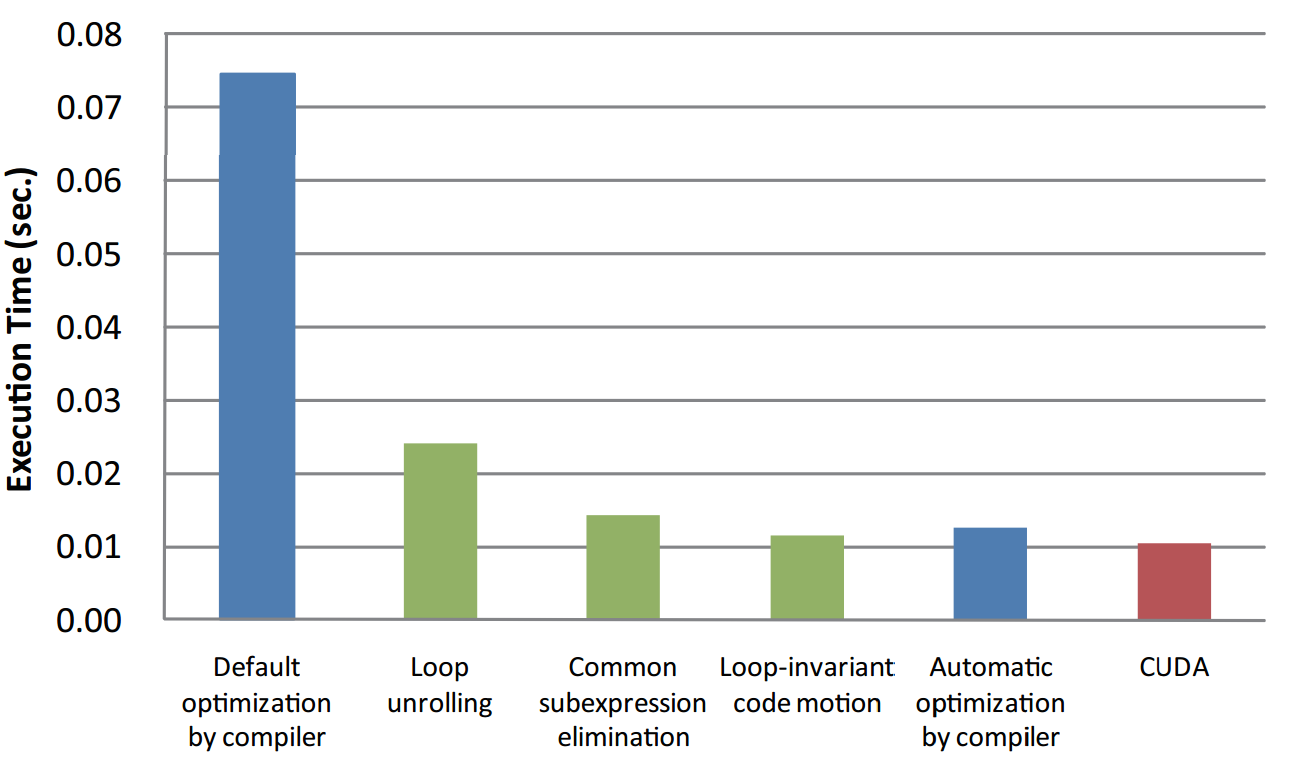
\includegraphics[width=1\textwidth]{figures/opencloptimisation.png} % trim=4.85cm 15cm 0.85cm 1cm
\caption{Execution speed of a matrix multiplication with different increases in runtime efficiency done. \todo[inline]{Det ville være TRIVIELT at forklare hvad disse optimeringer er og hvorfor programmet er hurtere på grund af det. Skal vi det? -- Troels} \citep{CUDAOpenCLOptimisation}}\label{image:OpenCLOptCompare}
\vspace{-15pt}
\end{figure}
\todo[inline]{dette er plagiat. Det skal tydeligt fremgå det ikke er vores billede. MP - Det fremgår da også rimelig tydeligt i det at der er en kilde på billedet? - Marc}
As seen on \myref{image:OpenCLOptCompare} some possible methods of increasing runtime efficiency includes loop unrolling, common sub-expression elimination and loop-invariant code motion. 
These are taken as specific examples in this comparison because these methods are performed in the \acrfull{ptx} code that CUDA compiles to. %ENDING A SENTENCE WITH A PROPOSITION OMG!!!
An OpenCL C compiler will also increases the runtime efficiency of the source code if given the instruction to, however its impact depends on the \acrshort{gpu} and platform in use.
The value of any increases in runtime efficiency is situational, i.e. changing the work-group size can yield improvements of up to 5 times. \citep{ocl_lecture3}
OpenCL can use \acrshort{jit} to generate binary code to the appropriate device it is working with at runtime.
This allows OpenCL to increases in runtime efficiency for the \acrshort{gpu} used, however this is also a constant overhead for each execution of the program. 
OpenCL can also compile the kernels before runtime, this is known as an offline compilation as opposed to the \acrshort{jit} compilation known as online compilation. 
The CUDA compiler \texttt{nvcc} is a two step process, which first generates \acrshort{ptx} bytecode and then either \acrshort{jit} compile on runtime or compiles a so called ``fat binary''at compile time, which contains multiple programs for different \acrshort{gpu}s. \citep{nvidia_cude_fat_bin}

%Optimising C code(CPU)
As \gls{gamble} does not exclusively perform its operations on the \acrshort{gpu} the code run on the \acrshort{cpu} must also be considered as a point in which runtime efficiency can be increased.
Some methods of increasing runtime efficiency on the \acrshort{cpu} are similar as mentioned earlier such as loop unrolling.\todo{Skal vi evt. forklare hvad det er ?? - Søren Er enig, men måske er det for trivielt? At forklare det vil dog vise vores kendskab til det. -- Troels}
Further methods pertain to the architectural differences between \acrshort{cpu}s and \acrshort{gpu}s, in particular cache- and pipeline-friendly code.
Cache-friendly code means considering the principle of spatial locality i.e. memory regions closer to each other, are more likely to be accessed within a short time.
To write pipeline-friendly code one must in particular consider branch prediction, however the best way is simply to avoid branching. \citep{CCodeOpt}
While these methods may very well increase runtime efficiency, there is no reason to implement them as the GNU Compiler Collection (GCC) already implements well developed methods of increasing runtime efficiency beyond our abilities.
\begin{figure}
\centering
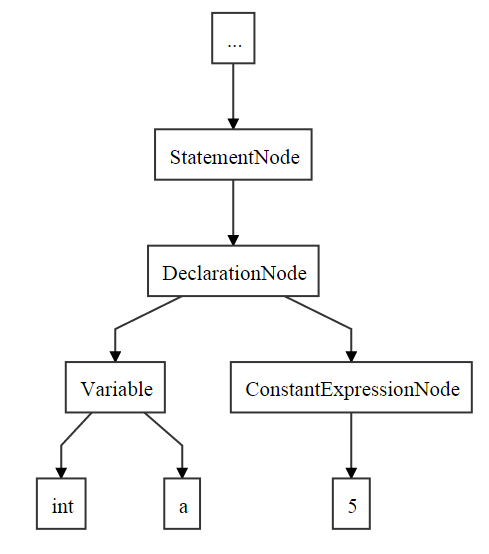
\includegraphics[width=0.5\textwidth]{figures/Trees/ASTAlone.PNG}
\caption{An \acrshort{ast} for the declaration \texttt{int a = 5;}}\label{fig:ASTAlone}
\end{figure}

\myref{fig:ASTAlone} shows a \texttt{DeclarationNode} for the expression \texttt{int a = 5;}. 
In the code generator this node will be transformed into the declaration written in C. 
The syntax for this is actually the same in C as it is in \gls{gamble}. 
The node has been through the previous phases, type and scope check, and is therefore ready to be computed.
The code executed when the visitor accepts a \texttt{DeclarationNode} can be seen on \myref{lst:DeclarationNodeCodeGen}.
\begin{lstlisting}[float, floatplacement=H!, caption=The visit method for visitting a DeclarationNode in the codegenerator. ,frame=tlrb,label={lst:DeclarationNodeCodeGen}]
@Override
public String VisitDeclarationNode(DeclarationNode node) {
    String expr = "";
    String complexType = "";
    if (node.getExpression() != null){
        resultVarStack.push(node.getVariable());
        expr = visit(node.getExpression());
        resultVarStack.pop();
    }

    if (node.getVariable().isComplex()) {
        ...
    }
    if (expr.indexOf("sclManageArgsLaunchKernel
    	(hardware, software, global_size, local_size") >= 0){
        ...
    }
    
    return complexType.length() > 0 ? complexType + expr : 
    (node.getVariable().toCcode() + " = " + expr + ";");
}
\end{lstlisting}
Since the example \texttt{int a = 5;} is not of a complex data type like a matrix or vector the body of the second and third if statements are hidden.\todo{Måske vise den i bilag hvor den ikke er hidden?}
A method is called on the node to check whether the expression that assigned the declared variable exists. 
Syntactically a matrix or vector may appear to be uninitialised but this actually creates a vector or matrix filled with zeros.
In \myref{lst:DeclarationNodeCodeGen} the expression is not null so it enters the body of the \texttt{if} statement on line 5.
The result variable, which stores the result of the expression, is pushed to a stack before visiting the expression.
In the method \texttt{VisitExpresssionNode} the top of the stack, which the result was pushed to, is checked to see if the result is a complex datatype or not; in the example the result is not of a complex data type and the expression is then evaluated by visiting the nodes of the expression.
The result of the call to \texttt{VisitExpressionNode} is saved to a string \texttt{expr}.
Another if statement checks if the declaration needs a kernel and if the expression needs to be computed on the \acrshort{gpu}.
When the call to \texttt{VisitDeclarationNode} returns; it is checked whether the string \texttt{complexType} has been made longer or not.
In the example \texttt{int a = 5;} it has not and therefore the string of the datatype and ID are concatenated with the assignment symbol, the substring \texttt{expr} and a semi-colon, before finally being returned.






In the following section an introduction of a library called SimpleOpenCL will take place.
\subsubsection*{Using SimpleOpenCl}
Simple\gls{opencl} is a library for C which simplifies the process of setting up and launching a kernel for \gls{opencl}.
The kernels remain the same, but finding the hardware for executing the kernels and allocating memory for the hardware is simplified.

The \texttt{CodeGeneraterVisitor} starts at the root of the \acrshort{ast} and here the code on \myref{lst:OpenCLSetup} is run.

\begin{lstlisting}[caption=Call to setup Simple\gls{opencl} in the compiler by appending it to a string builder,numbers=none,frame=tlrb,label={lst:OpenCLSetup}]
outputCode.append(filesNstuff.
	 ImportStringFromResource("codesnippets/simpleCLsetup.c") + "\n\n");
\end{lstlisting}
The file simpleCLsetup.c is appended to the code right as the main method of the output file is started.
The file contains the code which can be seen on \myref{lst:OpenCLSetup2}.

\begin{lstlisting}[caption=Simple\gls{opencl} setup in the compiler,numbers=none,frame=tlrb,label={lst:OpenCLSetup2}]
// Simple-\gls{opencl} Hardware setup
	sclHard* allHardware;
	sclHard hardware;
	sclSoft software;
	int found = 0;
	allHardware = sclGetAllHardware( &found );
	hardware = sclGetFastestDevice(allHardware, found);

    size_t local_size[2] = {1, 1};
    size_t global_size[2] = {1, 1}; 

    printf("\n");
// END Hardware setup
\end{lstlisting}

This code creates the elements needed to launch a kernel.
It finds the fastest hardware according to SimpleOpenCl's function calls, which means it finds the device with the most number of compute units, no matter the type of device, be it a \acrshort{cpu} or a \acrshort{gpu}.
For the remaining part of this section the fastest device is a \acrshort{gpu}.
\texttt{global\_size} and \texttt{local\_size} are there to determine the amount of memory needed both globally and locally on the \acrshort{gpu}.
The size of these arrays are initialised to two, because the \gls{gamble} matrices are two-dimensional.
These arrays are then filled out with different numbers corresponding to the columns and rows of the matrices or vectors being calculated upon.
This way of appending templates to the outputCode string is used in different places in the code generation when handling the complex datatypes matrices and vectors.
In fact whenever one of the following operators \texttt{+, -, *, \#, \^{} } are used with matrices or vectors a template is being appended to the outputCode. 
See \myref{tbl:matOps} for a description of what each operator will produce in \gls{gamble}.

When the right side of an assignment or declaration consists of an expression using operators and matrices or vectors, the visitor checks which operator is used and then inputs a template for launching the kernel depending on the operator.
The compiler contains files which have the code for launching the kernel for the specific situation and also for the kernel itself.
If a kernel is used the kernel file is added to the ``codeout'' directory along with the output code itself.

\myref{lst:kernelLaunch} shows one of the kernels being appended to the outputCode.

\begin{lstlisting}[caption=Simple\gls{opencl} launch of a kernel calculating a matrix or vector multiplied with a scalar.,numbers=none,frame=tlrb,label={lst:kernelLaunch}]
//MATRIX §MATRIX_A§ MULTIPLIED WITH A SCALAR §MATRIX_B§
global_size[0] = §MATRIX_A§.rows*§MATRIX_A§.cols;
local_size[0] = 1;
global_size[1] = 1;
local_size[1] = 1;
software = sclGetCLSoftware("matrixMulScalar.cl", "matrixMulScalar", hardware);
§MATRIXTYPE§ scl_scalar_mul§NUM§ = §MATRIX_B§;
// %R means that what is being sent can be read from and written to
// %a means that what is being sent is a non-pointer argument and is constant
sclManageArgsLaunchKernel(hardware, software, global_size, local_size, "%R %a",
    §MATRIX_A§.dataSize, §MATRIX_A§.dataStart, sizeof(§MATRIXTYPE§), &scl_scalar_mul§NUM§);
//END MATRIX SCALAR MULTIPLY
\end{lstlisting}

\texttt{global\_size} is set to be the size of the matrix, and a kernel is then launched for every index in the matrix.
This is decided by setting the indices in \texttt{global\_size}.
If the squared matrix was 2x2, a kernel would be launched with 0, 1, 2 and 3 as the indices.
The implementation of multiplying a matrix with a scalar is made where the matrix is interpreted as a single vector where each row comes after the other.
If the matrix form is needed the rows of the matrix would be placed in \texttt{global\_size[0]} and the columns in \texttt{global\_size[1]}.
If the example of a size 4 matrix is still used, the following sets of kernels would be sent:
\begin{equation}
\{0,0\}, \{0,1\}, \{1,0\}, \{1,1\}
\end{equation}
So a kernel for each index in the matrix.
This can then be used in the kernel to determine which row and which column, the index being sent to the kernel for execution, possess.
The \texttt{software} is where the kernel being launched is set, the file name and the kernel name in the file, the hardware for the execution must also be set.
Then the function \texttt{sclManageArgsLaunchKernel()} handles the launching itself with the variables needed to launch the kernel.
Before this code is appended any string with  \S-signs is is replaced by the corresponding string depending on the situation.
So \texttt{§MATRIX\_A§} is replaced with the id of the left matrix in the expression node.
The code for replacing the strings can be seen on \myref{lst:replaceString}.

\begin{lstlisting}[caption=Code for replacing strings with the corresponding information to be appended to the outputCode.,numbers=none,frame=tlrb,label={lst:replaceString}]
private String matrixKernel(String kernelName, String aID, String bID, String resID, String simpleType) {
    String kernel = filesNstuff.ImportStringFromResource("kernels/" + kernelName + ".cl");
    kernel = kernel.replaceAll("§MATRIXTYPE§", simpleType);
    filesNstuff.WriteToFile(new File("../../../codeout/" + kernelName + ".cl"), kernel);

    String argsNlauch = filesNstuff.ImportStringFromResource("kernelLaunch/" + kernelName + ".c");
    argsNlauch = argsNlauch.replaceAll("§MATRIX_A§", aID);
    argsNlauch = argsNlauch.replaceAll("§MATRIX_B§", bID);
    argsNlauch = argsNlauch.replaceAll("§MATRIX_RES§", resID);
    argsNlauch = argsNlauch.replaceAll("§MATRIXTYPE§", simpleType);
    argsNlauch = argsNlauch.replaceAll("§NUM§", Integer.toString(this.scalarNum));
    argsNlauch = argsNlauch.replaceAll("\\n", "\n" + indent(""));
    return argsNlauch;
}
\end{lstlisting}

However this must also be done for the kernel itself, in the kernels the type is changed depending on the type of the fields in the matrix or vector, which makes it possible to use the same code in the code generator for replacing these strings, since the type is handled dynamically.

The corresponding kernel for \myref{lst:kernelLaunch} can be seen on \myref{lst:kernel}.
\begin{lstlisting}[caption=Kernel code for multiplying a matrix or vector with a scalar.,numbers=none,frame=tlrb,label={lst:kernel}]
__kernel void matrixMulScalar(__global §MATRIXTYPE§ *ma, §MATRIXTYPE§ scalar){
	int global_x = get_global_id( 0);
	ma[ global_x] *=  scalar;
}
\end{lstlisting}

As can be seen the string \texttt{§MATRIXTYPE§} must also be replaced here.
The index which has been sent to the kernel is retrieved by calling \texttt{get\_global\_id(0);}.
The index is then used to access the matrix at the specific index and multiply the value at the index with the scalar.


\subsubsection*{From OpenCL to execution}\label{makefile}
After the \gls{gamble} compiler have compiled the source code; the compiler outputs OpenCL C code as its object code.
The OpenCL C code must be compiled by a C-compiler such as the GCC (GNU Compiler Collection) compiler to produce code the \acrshort{cpu} and \acrshort{gpu} can execute.
During the compilation the OpenCL C headers must be accessable, to provide the functions and types used. 
Aditionally the \gls{gamble} standard libary, containing functions such as \texttt{matrixToFile} and \texttt{fileToMatrix} must also be included and compiled. 
This produces an executable file for the platform targetted by the compiler, this will most often be the platform running, such as x86--64 on Linux.
The same executeable file is not usable for another platform, e.g. ARM, nor on another operating system, e.g. Windows or OS X.\todo{Skal vi ændre dette til OS X only med gamble?}
To maintain portability a ``MakeFile'' is used; a MakeFile is a file in the syntax which the GNU make utility can execute. 
The make utiliry is a set of rules which ensures that the correct compiler, path, headers, etc. are used during compilation on one of multiple platforms. 
This means that after running the \gls{gamble} compiler, on a configured computer, e.g. has OpenCL C headers, libary, a compiler etc., the make command can be used to build a binary file to be executed.

The kernel can either be compiled at compile-time or \acrshort{jit} compiled at runtime.
The JIT compilation, called online compilation under OpenCL, allows the system to adapt with platform specific optimisations for the running platform.
If the kernel is compiled at compile-time, called offline compilation under OpenCL, then it might support fewer devices, or will take a long time and increase the size of the executable as it has to contain versions for each hardware for which support is requested. \citep{openclbookjit}
For \gls{gamble} the online compilation is chosen for its simplicity as it lets the driver of the running system compile the kernel. 

A typical compilation on Ubuntu 14.04 configured with OpenCL headers located at \path{/opt/opencl-headers/include/} will look like \myref{lst:makecommands}, where \texttt{code.c} is the output of the \gls{gamble} compiler.
After the execution of these, an output file called \texttt{run} is made and can be executed with the command \texttt{./run}. 

\begin{lstlisting}[caption=The commands executed by the make command according to the rules of the MakeFile,numbers=none,frame=tlrb,label={lst:makecommands}]
gcc -Wall -Wextra -pedantic -O3 -std=c99 -I/opt/opencl-headers/include/ -c code.c simpleCL.c gambleStdlib.c
gcc -Wall -Wextra -pedantic -O3 -std=c99 *.o -o run -lm -lOpenCL -lrt
rm -f *.o
\end{lstlisting}
